\section{Methodology}

\begin{enumerate}
	\item 4 shots of grid: 1. LE 2. TE 3. near-field for entire shape 4. the entire grid domain. Note: should show T-rex feature that was used
	\item table 1: cell count and normal-to-wall spacing used, list BC, list reference values, list submodels chosen (i.e. viscous model), provide numerical scheme and spacial accuracy
	
\subsection{Screenshots of grid}

\begin{figure}[ht]
	\centering
	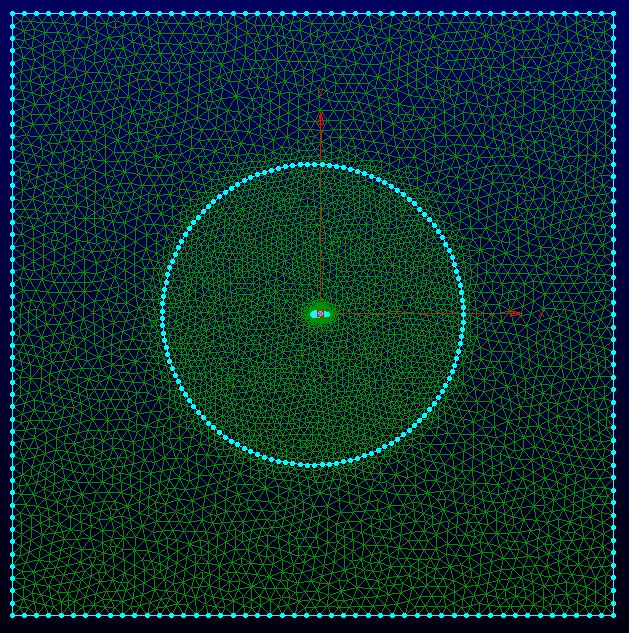
\includegraphics[width=\textwidth]{general_images/farfield}
	\caption{Farfield}
\label{fig:farfield}
\end{figure}

\begin{figure}[ht]
	\centering
	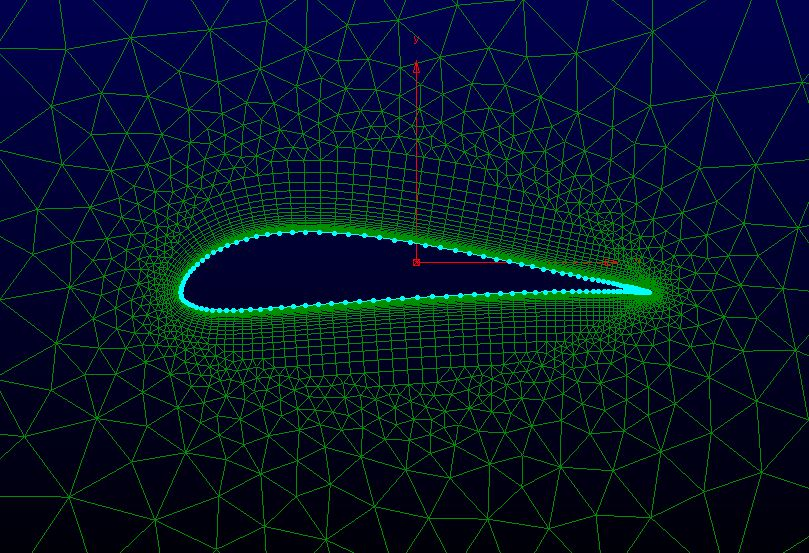
\includegraphics[width=\textwidth]{general_images/nearfield}
	\caption{Nearfield}
\label{fig:nearfield}
\end{figure}	

\begin{figure}[ht]
	\centering
	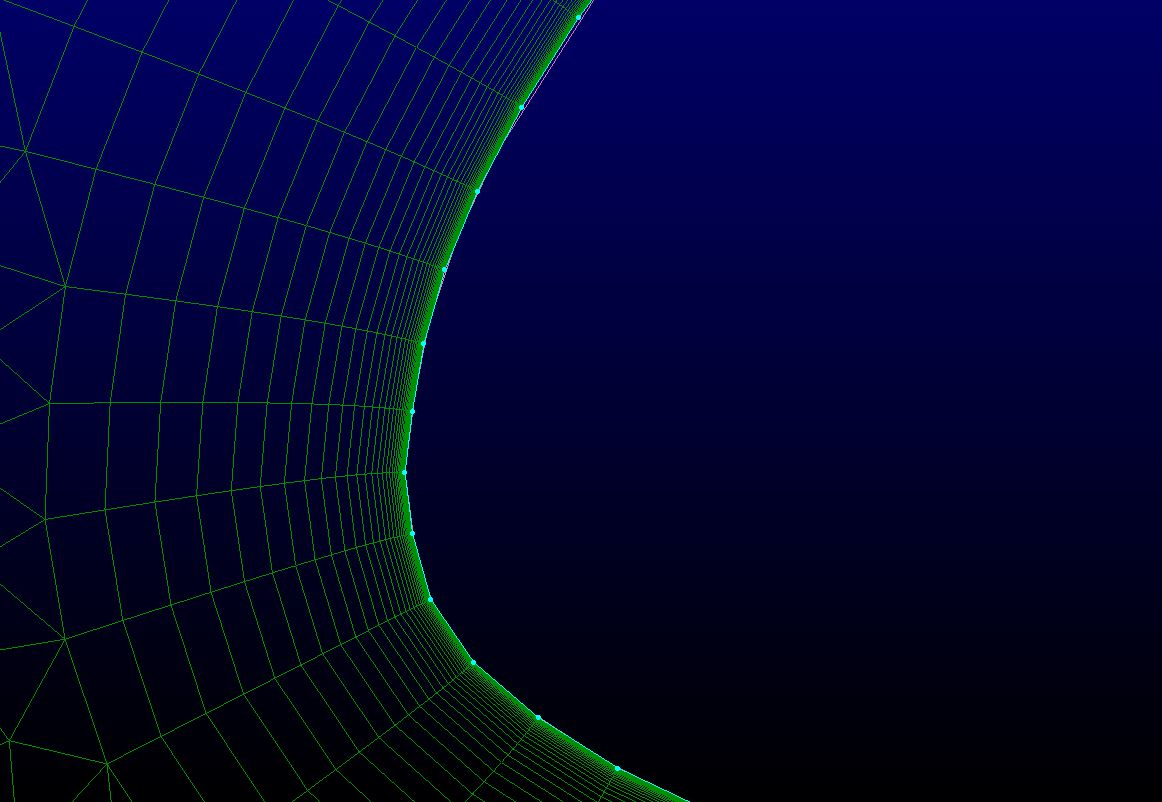
\includegraphics[width=\textwidth]{general_images/LE1}
	\caption{Leading edge}
\label{fig:LE}
\end{figure}

\begin{figure}[ht]
	\centering
	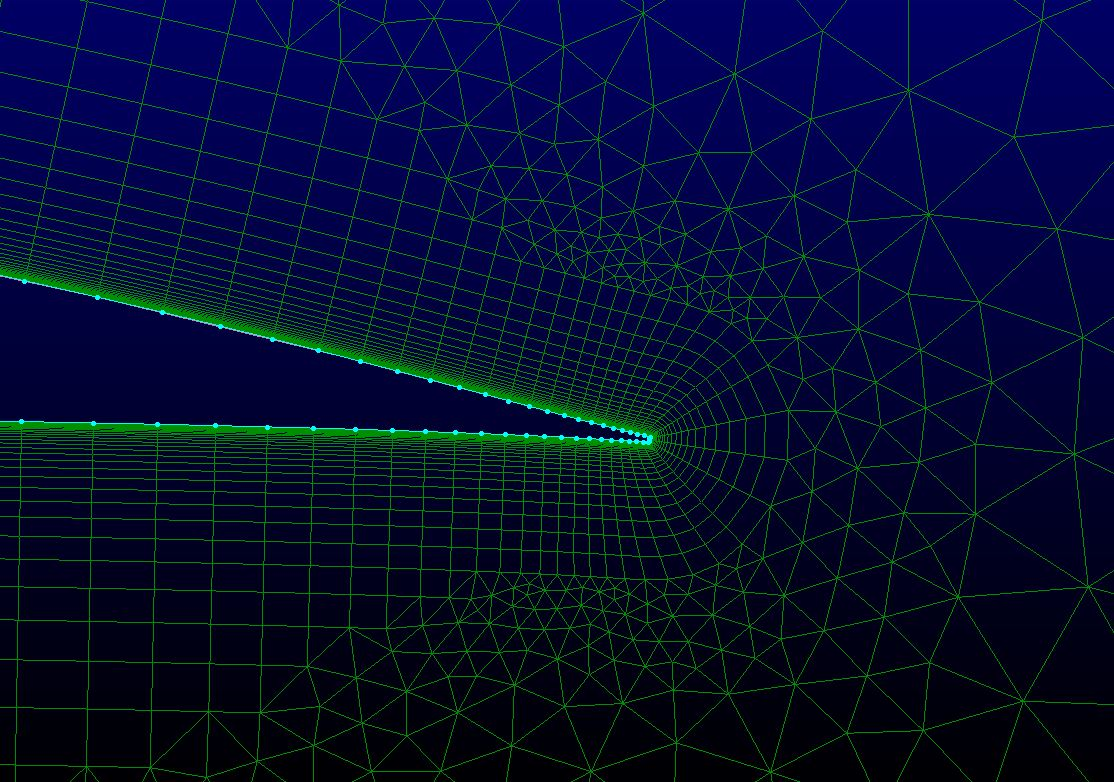
\includegraphics[width=\textwidth]{general_images/TE1}
	\caption{Trailing edge}
\label{fig:TE}
\end{figure}
		
\end{enumerate}